\documentclass{beamer}
\usepackage[utf8]{inputenc}
\usepackage{microtype}
\usepackage{siunitx}
\newcommand{\GR}{{GNU\,Radio}}
\usetheme{GNURadio}
\title[GNU Radio -- SDR for the masses]{GNU Radio}
\subtitle{SDR for the masses}
\author{Marcus Müller}
%\institute{Ettus Research}
\date{Software Defined Radio Academy 2015}
\subject{Software Defined Radio}
\begin{document}
\frame{\titlepage}


%%%%%%%%%%%%%%%%%%%%%%%%%%%%%%%%%%%%%%%%%%%%%%%%%%%%%%%%%%%%%%%%%%%%%%%%%%%%%
\section{Introduction}
%%%%%%%%%%%%%%%%%%%%%%%%%%%%%%%%%%%%%%%%%%%%%%%%%%%%%%%%%%%%%%%%%%%%%%%%%%%%%

\begin{frame}{Who am I?}
  \begin{itemize}
    \item GNU Radio contributor and user
    \item Spent too much time on the \texttt{discuss-gnuradio@gnu.org} mailing list
    \item Got hired by \,\includegraphics[height=2em]{ettuslogo.png}
  \end{itemize}
  \pause
  \ldots and who is Ettus?
  \begin{itemize}
    \item Producer of the USRP series of SDR frontends\\
    \item \texttt{gr-uhd} integrates directly in GNU Radio
    \item \texttt{http://www.ettus.com}
  \end{itemize}
\end{frame}

\begin{frame}{A short overview}
  \tableofcontents{}
\end{frame}

%%%%%%%%%%%%%%%%%%%%%%%%%%%%%%%%%%%%%%%%%%%%%%%%%%%%%%%%%%%%%%%%%%%%%%%%%%%%%
\section{What is GNU Radio}
%%%%%%%%%%%%%%%%%%%%%%%%%%%%%%%%%%%%%%%%%%%%%%%%%%%%%%%%%%%%%%%%%%%%%%%%%%%%%

\begin{frame}{What is GNU Radio?}
  \dots and more importantly: \emph{Why would I want that?}
\end{frame}

\begin{frame}{A Sample Flow Framework}
  Radio signal processing often looks like a chain of steps:

  \vfill
  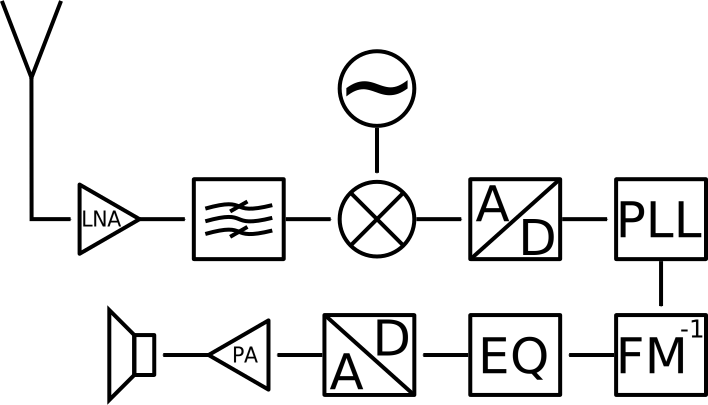
\includegraphics[width=\textwidth]{carrx.pdf}
\end{frame}
\begin{frame}{A Sample Flow Framework}

  GNU Radio is a signal flow graph oriented framework:

 \vfill
 \includegraphics[width=\textwidth]{carrxfg.png}

\end{frame}

\begin{frame}{GNU Radio comes with a toolbox of useful blocks}
\begin{itemize}
  \item hardware interface blocks
  \item basic mathematical operations
  \item filters
  \item digital modulators
  \item analog modulators
  \item network tools
  \item example implementations (digital TV, pagers, Sat images\ldots)
  \item \dots
\end{itemize}

\dots \textbf{But it's not a receiver/transmitter for any particular standard.}
\end{frame}

\begin{frame}{What people built with GNU Radio}
  GNU Radio can rely on an active community with many useful modules, among those
  \begin{itemize}
  \item GQRX
  \item gr-radar
  \item gr-ieee802-11
  \item and much more
  \end{itemize}
  Have a look at CGRAN, \url{http://cgran.org}
\end{frame}

\begin{frame}{GNU Radio has an application installer!}
  PyBOMBS: convenient installer for GNU Radio, build dependencies and out-of-tree modules

  \includegraphics[height=16em]{pybombs.png}\centering
\end{frame}

%%%%%%%%%%%%%%%%%%%%%%%%%%%%%%%%%%%%%%%%%%%%%%%%%%%%%%%%%%%%%%%%%%%%%%%%%%%%%
\section{Core Concepts}
%%%%%%%%%%%%%%%%%%%%%%%%%%%%%%%%%%%%%%%%%%%%%%%%%%%%%%%%%%%%%%%%%%%%%%%%%%%%%

\begin{frame}{Core concept: Block}
  A block represents a signal processing step

  \includegraphics{block.png}\centering

  \begin{itemize}
    \item can have 0 or more inputs
    \item can have 0 or more outputs
    \item can either
      \begin{itemize}
        \item do its own signal processing
        \item or contain different blocks in itself
      \end{itemize}
  \end{itemize}
\end{frame}


\begin{frame}{Core concept: Item Stream}
  A stream is the connection between two blocks

  \includegraphics{stream.png}\centering

  \begin{itemize}
    \item data is exchanged between blocks on predefined connections, \emph{streams}
    \item these streams represent the output buffer of the producing block, and
    \item the input buffer(s) of the consuming block(s)
  \end{itemize}
\end{frame}


\begin{frame}{Core concept: Flow Graph}
  A Flow graph is the abstract representation of how GNU Radio connects different blocks


  \includegraphics[height=15em]{rxofdm.png}

\end{frame}

%%%%%%%%%%%%%%%%%%%%%%%%%%%%%%%%%%%%%%%%%%%%%%%%%%%%%%%%%%%%%%%%%%%%%%%%%%%%%
\section{Typical Work Flow 1: Flow graphs in GRC}
%%%%%%%%%%%%%%%%%%%%%%%%%%%%%%%%%%%%%%%%%%%%%%%%%%%%%%%%%%%%%%%%%%%%%%%%%%%%%

\begin{frame}{Let's build a Demo!}
Observing the whole LDP433 spectrum
\begin{itemize}
  \item 25 channels, \SIrange{433.075}{434.775}{\mega\hertz}
  \item channel spacing: \SI{25}{\kilo\hertz}
  \item Modulation: FM
  \item receiving and visualizing the whole spectrum
  \item demodulation and playback of a single channel
\end{itemize}
\end{frame}
\begin{frame}{Spectrum Visualizer}
  \only<1>{\includegraphics[width=\textwidth]{rxdemo.png}}
  \only<2>{\includegraphics[width=\textwidth]{rxfg.png}}
\end{frame}

\begin{frame}{Demo: What's happening behind the scenes?}
    \begin{itemize}
      \item GNU Radio Companion (GRC) converts graphically defined flow graph to python file
      \item As python gets executed, blocks get instantiated and connections defined by calling GNU Radio methods
      \item The flow graph is started: GNU Radio starts calling the blocks' \texttt{work} methods
      \item \texttt{work} methods consume input and produce output
      \item GNU Radio calls the surrounding blocks again, now that there's new output space / new input
    \end{itemize}
\end{frame}
\begin{frame}{What's happening in the individual blocks?}
  \includegraphics[width=\textwidth]{rxfg.png}
\end{frame}

%%%%%%%%%%%%%%%%%%%%%%%%%%%%%%%%%%%%%%%%%%%%%%%%%%%%%%%%%%%%%%%%%%%%%%%%%%%%%
\section{The USRP B2x0: A direct mixing SDR architecture}
%%%%%%%%%%%%%%%%%%%%%%%%%%%%%%%%%%%%%%%%%%%%%%%%%%%%%%%%%%%%%%%%%%%%%%%%%%%%%

\begin{frame}{What's happening on the hardware side of things?}
  The Ettus USRP B210 is the interface between software and RF:\bigskip


  \includegraphics[width=\textwidth]{whatusrp.pdf}
\end{frame}
\begin{frame}{Features of the B200/B210}
\begin{description}
  \item[Channels] B200: 1 TX \& 1 RX, B210: 2 TX \& 2 RX
  \item[Coverage] Seamless \SI{70}{\mega\hertz} to \SI{6}{\giga\hertz}
  \item[$f_\text{ADC}$] flexible, up to \SI{56}{\mega\hertz}
  \item[user $f_\text{sample}$] flexible, $\frac{f_\text{ADC}}{N}, N \in 1,\dots,512$
  \item[Duplex] Full duplex
  \item[Analog Filters] Adjustable, up to $f_\text{sample}$
  \item[Digital Filters] Automatically chosen to optimize signal
  \item[Connectivity] USB3
  \item[Host Driver] Open Source, \url{https://github.com/EttusResearch/uhd/}
  \item[Firmware] Open Source
  \item[FPGA] Open Source
  \item[Schematics] Online, \url{http://files.ettus.com/schematics/b200/}
\end{description}
\end{frame}
\begin{frame}{structure of the B2x0 direct receiver}
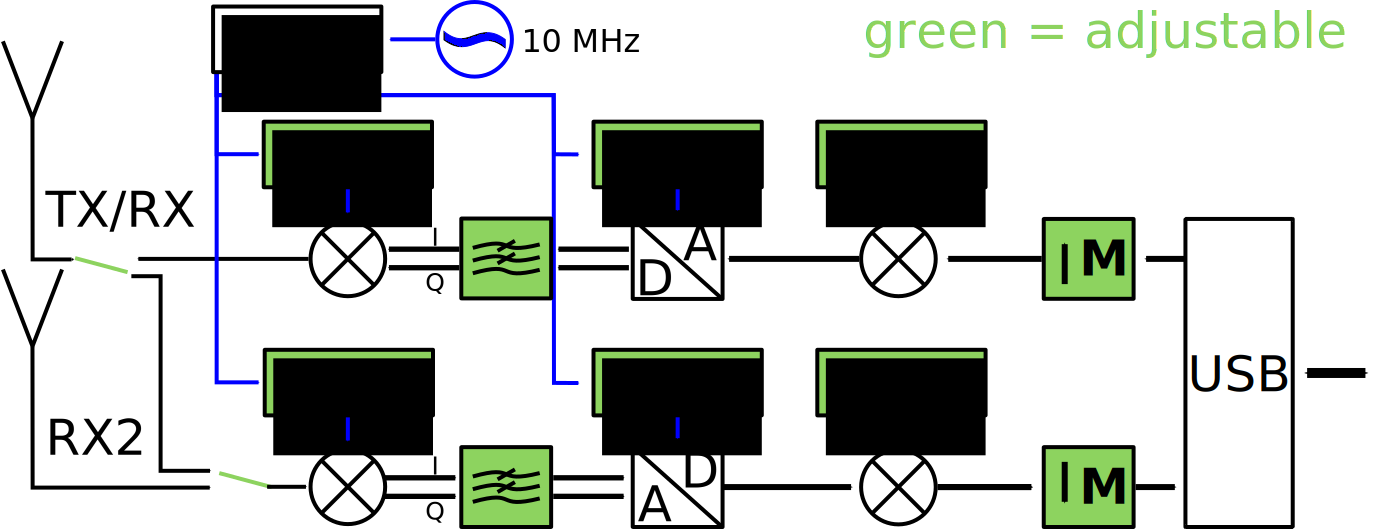
\includegraphics[width=\textwidth]{b200.pdf}
\end{frame}

%%%%%%%%%%%%%%%%%%%%%%%%%%%%%%%%%%%%%%%%%%%%%%%%%%%%%%%%%%%%%%%%%%%%%%%%%%%%%
\section{Questions and Answers}
%%%%%%%%%%%%%%%%%%%%%%%%%%%%%%%%%%%%%%%%%%%%%%%%%%%%%%%%%%%%%%%%%%%%%%%%%%%%%
\begin{frame}{Questions? Answers!}
  Now is the time for some questions and some answers, before we move on.
\end{frame}

%%%%%%%%%%%%%%%%%%%%%%%%%%%%%%%%%%%%%%%%%%%%%%%%%%%%%%%%%%%%%%%%%%%%%%%%%%%%%
\section{Typical Work Flow 2: How to build a talking clock}
%%%%%%%%%%%%%%%%%%%%%%%%%%%%%%%%%%%%%%%%%%%%%%%%%%%%%%%%%%%%%%%%%%%%%%%%%%%%%
\begin{frame}{Demo: A talking clock}
  \begin{description}
    \item[What?] A clock that, every N seconds, says the current time.\pause
    \item[How?] Using an existing text-to-speech program and python blocks.\pause
    \item[Why?] Yes.
  \end{description}
\end{frame}
\begin{frame}{Design Approach}
  \begin{itemize}
    \item Using existing blocks, we can 
      \begin{itemize}
        \item Have an interface to the USRP
        \item Generate FM out of audio samples
        \item Have control over volume
      \end{itemize}
    \item What we still need is a block that generates the voice samples
      \begin{itemize}
        \item \texttt{itemize} is an established Text-to-Speak program
        \item we need to prepend the message with a ``ping''
      \end{itemize}
  \end{itemize}
\end{frame}
\begin{frame}{Step I: Constructing a flow graph with missing components}
  \includegraphics[width=\textwidth]{clockfg.png}
\end{frame}
\begin{frame}{Step II: Adding a python block stub}
  \texttt{gr\_modtool} allows us to create a module, and add a block stub:\bigskip\pause

  \hspace{3em}\fbox{\parbox{0.7\textwidth}{
    \texttt{gr\_modtool newmod talkingclock\\[0.1em]
      {\scriptsize\color{darkgray}{Creating out-of-tree module in ./gr-speakingclock\ldots Done.\\
      >Use 'gr\_modtool add' to add a new block to this currently empty module.}}}\\
  \texttt{cd gr-talkingclock}\\
  \texttt{gr\_modtool add\\
 {\scriptsize\color{darkgray}{GNU Radio module name identified: speakingclock\\
Enter block type: source\\
Language (python/cpp): python\\
\ldots}}}
}}

\end{frame}
\begin{frame}{Step III: Adding functionality}
  \begin{itemize}
    \item Most important about our block is the \texttt{work} method:
      \begin{itemize}
        \item gets called repeatedly
        \item has the job of filling the output buffer, and returning how many output items were produced
      \end{itemize}
    \item We add \texttt{tx\_time} and start-of-burst \emph{stream tags} so that the USRP knows when to transmit
    \item in the constructor, we make sure everything is set up correctly
  \end{itemize}
\end{frame}
\begin{frame}{Step IV: Putting it all together}
  \includegraphics[width=\textwidth]{clockaudiofg.png}
\end{frame}


%%%%%%%%%%%%%%%%%%%%%%%%%%%%%%%%%%%%%%%%%%%%%%%%%%%%%%%%%%%%%%%%%%%%%%%%%%%%%
\section{Useful Resources}
%%%%%%%%%%%%%%%%%%%%%%%%%%%%%%%%%%%%%%%%%%%%%%%%%%%%%%%%%%%%%%%%%%%%%%%%%%%%%
\begin{frame}{Useful Links}
  \begin{description}
    \item[GNU Radio project] \url{http://gnuradio.org}
    \item[Guided Tutorials] \url{https://gnuradio.org/redmine/projects/gnuradio/wiki/Guided_Tutorials}
    \item[CGRAN] \url{http://cgran.org}
    \item[PyBOMBS]\url{http://pybombs.info}\\[1.5em]
    \item[GNU Radio mailing list] \href{mailto:discuss-gnuradio@gnu.org}{discuss-gnuradio@gnu.org}\\
      Registration \& Archive: \url{https://lists.gnu.org/mailman/listinfo/discuss-gnuradio}\\[1.5em]
    \item[Ettus] \url{http://www.ettus.com}
    \item[UHD Manual] \url{http://files.ettus.com/manual/}
  \end{description}
\end{frame}
\end{document}
